In this chapter, we utilize \demo{} in order to extend the evaluation of
PolderCast and Scribe found in~\cite{Setty:2012} on a set of topology
metrics. These metrics are afforded to us for ``free'' by the Gephi
framework through the Statistics API included in the \emph{Gephi
    Toolkit}.

\section{Experimental Setup}

We run PolderCast and Scribe in PeerNet using the simulation mode. The
Simulations consists of 1000 PeerNet cycles as well as 1000 reporter
intervals. We use workloads both from Facebook~\cite{} and
Twitter~\cite{} in order to model subscriptions. As mentioned in
Chapter~\ref{ch:vizpub}, the Facebook data trace include 3 million user
profiles along with 28.3 million friend relations. The Twitter dataset
consists of 41.7 million distinct users and 1.47 billion
follow/followed relations.

The social relations in Facebook are reciprocal, which leads us to model
bidirectional subscriptions. More specifically, a Facebook user is
modeled as a topic. The friends list of the particular user profile
constitutes its subscription list. All of the entries in this list will
include the original user in their own lists of subscriptions.
Relationships in Twitter however, are unidirectional. When using the
Twitter trace, users are also modeled as topics, but here the list of
subscriptions are formed on the basis of the ``following'' list of the
particular  user profile. The entries in this list are not required to
follow back, therefore subscriptions are also unidirectional.

Churn is based on the Skype super-peer trace from~\cite{}, tracing 4000
nodes for 4 weeks, tracking their joining and leaving timestamps. We
scale churn to include the first day of this trace in order to not
introduce a churn rate which is unrealistically high. For latency
between node pairs, we use the King dataset found in~cite{}.

\section{Experimental Restrictions}

\section{Results}

\begin{figure}
    \centering
    % GNUPLOT: LaTeX picture with Postscript
\begingroup
  \makeatletter
  \providecommand\color[2][]{%
    \GenericError{(gnuplot) \space\space\space\@spaces}{%
      Package color not loaded in conjunction with
      terminal option `colourtext'%
    }{See the gnuplot documentation for explanation.%
    }{Either use 'blacktext' in gnuplot or load the package
      color.sty in LaTeX.}%
    \renewcommand\color[2][]{}%
  }%
  \providecommand\includegraphics[2][]{%
    \GenericError{(gnuplot) \space\space\space\@spaces}{%
      Package graphicx or graphics not loaded%
    }{See the gnuplot documentation for explanation.%
    }{The gnuplot epslatex terminal needs graphicx.sty or graphics.sty.}%
    \renewcommand\includegraphics[2][]{}%
  }%
  \providecommand\rotatebox[2]{#2}%
  \@ifundefined{ifGPcolor}{%
    \newif\ifGPcolor
    \GPcolortrue
  }{}%
  \@ifundefined{ifGPblacktext}{%
    \newif\ifGPblacktext
    \GPblacktexttrue
  }{}%
  % define a \g@addto@macro without @ in the name:
  \let\gplgaddtomacro\g@addto@macro
  % define empty templates for all commands taking text:
  \gdef\gplbacktext{}%
  \gdef\gplfronttext{}%
  \makeatother
  \ifGPblacktext
    % no textcolor at all
    \def\colorrgb#1{}%
    \def\colorgray#1{}%
  \else
    % gray or color?
    \ifGPcolor
      \def\colorrgb#1{\color[rgb]{#1}}%
      \def\colorgray#1{\color[gray]{#1}}%
      \expandafter\def\csname LTw\endcsname{\color{white}}%
      \expandafter\def\csname LTb\endcsname{\color{black}}%
      \expandafter\def\csname LTa\endcsname{\color{black}}%
      \expandafter\def\csname LT0\endcsname{\color[rgb]{1,0,0}}%
      \expandafter\def\csname LT1\endcsname{\color[rgb]{0,1,0}}%
      \expandafter\def\csname LT2\endcsname{\color[rgb]{0,0,1}}%
      \expandafter\def\csname LT3\endcsname{\color[rgb]{1,0,1}}%
      \expandafter\def\csname LT4\endcsname{\color[rgb]{0,1,1}}%
      \expandafter\def\csname LT5\endcsname{\color[rgb]{1,1,0}}%
      \expandafter\def\csname LT6\endcsname{\color[rgb]{0,0,0}}%
      \expandafter\def\csname LT7\endcsname{\color[rgb]{1,0.3,0}}%
      \expandafter\def\csname LT8\endcsname{\color[rgb]{0.5,0.5,0.5}}%
    \else
      % gray
      \def\colorrgb#1{\color{black}}%
      \def\colorgray#1{\color[gray]{#1}}%
      \expandafter\def\csname LTw\endcsname{\color{white}}%
      \expandafter\def\csname LTb\endcsname{\color{black}}%
      \expandafter\def\csname LTa\endcsname{\color{black}}%
      \expandafter\def\csname LT0\endcsname{\color{black}}%
      \expandafter\def\csname LT1\endcsname{\color{black}}%
      \expandafter\def\csname LT2\endcsname{\color{black}}%
      \expandafter\def\csname LT3\endcsname{\color{black}}%
      \expandafter\def\csname LT4\endcsname{\color{black}}%
      \expandafter\def\csname LT5\endcsname{\color{black}}%
      \expandafter\def\csname LT6\endcsname{\color{black}}%
      \expandafter\def\csname LT7\endcsname{\color{black}}%
      \expandafter\def\csname LT8\endcsname{\color{black}}%
    \fi
  \fi
  \setlength{\unitlength}{0.0500bp}%
  \begin{picture}(7200.00,5040.00)%
    \gplgaddtomacro\gplbacktext{%
      \csname LTb\endcsname%
      \put(1342,704){\makebox(0,0)[r]{\strut{} 0.0001}}%
      \csname LTb\endcsname%
      \put(1342,1722){\makebox(0,0)[r]{\strut{} 0.001}}%
      \csname LTb\endcsname%
      \put(1342,2740){\makebox(0,0)[r]{\strut{} 0.01}}%
      \csname LTb\endcsname%
      \put(1342,3757){\makebox(0,0)[r]{\strut{} 0.1}}%
      \csname LTb\endcsname%
      \put(1342,4775){\makebox(0,0)[r]{\strut{} 1}}%
      \csname LTb\endcsname%
      \put(1474,484){\makebox(0,0){\strut{} 0}}%
      \csname LTb\endcsname%
      \put(1893,484){\makebox(0,0){\strut{} 100}}%
      \csname LTb\endcsname%
      \put(2311,484){\makebox(0,0){\strut{} 200}}%
      \csname LTb\endcsname%
      \put(2730,484){\makebox(0,0){\strut{} 300}}%
      \csname LTb\endcsname%
      \put(3148,484){\makebox(0,0){\strut{} 400}}%
      \csname LTb\endcsname%
      \put(3567,484){\makebox(0,0){\strut{} 500}}%
      \csname LTb\endcsname%
      \put(3985,484){\makebox(0,0){\strut{} 600}}%
      \csname LTb\endcsname%
      \put(4404,484){\makebox(0,0){\strut{} 700}}%
      \csname LTb\endcsname%
      \put(4822,484){\makebox(0,0){\strut{} 800}}%
      \csname LTb\endcsname%
      \put(5241,484){\makebox(0,0){\strut{} 900}}%
      \csname LTb\endcsname%
      \put(5659,484){\makebox(0,0){\strut{} 1000}}%
      \put(5791,704){\makebox(0,0)[l]{\strut{} 0}}%
      \put(5791,1111){\makebox(0,0)[l]{\strut{} 100}}%
      \put(5791,1518){\makebox(0,0)[l]{\strut{} 200}}%
      \put(5791,1925){\makebox(0,0)[l]{\strut{} 300}}%
      \put(5791,2332){\makebox(0,0)[l]{\strut{} 400}}%
      \put(5791,2740){\makebox(0,0)[l]{\strut{} 500}}%
      \put(5791,3147){\makebox(0,0)[l]{\strut{} 600}}%
      \put(5791,3554){\makebox(0,0)[l]{\strut{} 700}}%
      \put(5791,3961){\makebox(0,0)[l]{\strut{} 800}}%
      \put(5791,4368){\makebox(0,0)[l]{\strut{} 900}}%
      \put(5791,4775){\makebox(0,0)[l]{\strut{} 1000}}%
      \put(176,2739){\rotatebox{-270}{\makebox(0,0){\strut{}Avg. Clustering Coefficient}}}%
      \put(6692,2739){\rotatebox{-270}{\makebox(0,0){\strut{}Network Size}}}%
      \put(3566,154){\makebox(0,0){\strut{}Reporter Intervals}}%
    }%
    \gplgaddtomacro\gplfronttext{%
      \csname LTb\endcsname%
      \put(4672,1757){\makebox(0,0)[r]{\strut{}PolderCast (Facebook)}}%
      \csname LTb\endcsname%
      \put(4672,1537){\makebox(0,0)[r]{\strut{}PolderCast (Twitter)}}%
      \csname LTb\endcsname%
      \put(4672,1317){\makebox(0,0)[r]{\strut{}Scribe (Facebook)}}%
      \csname LTb\endcsname%
      \put(4672,1097){\makebox(0,0)[r]{\strut{}Scribe (Twitter)}}%
      \csname LTb\endcsname%
      \put(4672,877){\makebox(0,0)[r]{\strut{}Network Size}}%
    }%
    \gplbacktext
    \put(0,0){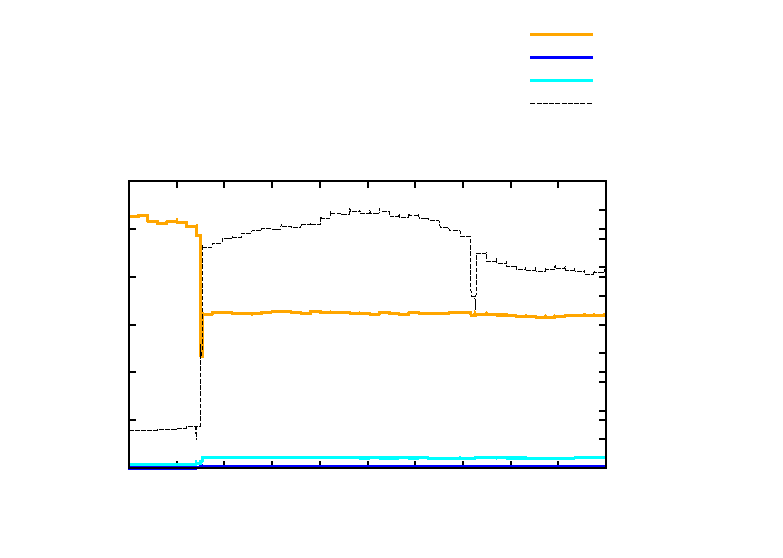
\includegraphics{eval_cc}}%
    \gplfronttext
  \end{picture}%
\endgroup

    \caption{Clustering Coefficient of PolderCast and Scribe}
    \label{fig:eval_cc}
\end{figure}

\begin{figure}
    \centering
    % GNUPLOT: LaTeX picture with Postscript
\begingroup
  \makeatletter
  \providecommand\color[2][]{%
    \GenericError{(gnuplot) \space\space\space\@spaces}{%
      Package color not loaded in conjunction with
      terminal option `colourtext'%
    }{See the gnuplot documentation for explanation.%
    }{Either use 'blacktext' in gnuplot or load the package
      color.sty in LaTeX.}%
    \renewcommand\color[2][]{}%
  }%
  \providecommand\includegraphics[2][]{%
    \GenericError{(gnuplot) \space\space\space\@spaces}{%
      Package graphicx or graphics not loaded%
    }{See the gnuplot documentation for explanation.%
    }{The gnuplot epslatex terminal needs graphicx.sty or graphics.sty.}%
    \renewcommand\includegraphics[2][]{}%
  }%
  \providecommand\rotatebox[2]{#2}%
  \@ifundefined{ifGPcolor}{%
    \newif\ifGPcolor
    \GPcolortrue
  }{}%
  \@ifundefined{ifGPblacktext}{%
    \newif\ifGPblacktext
    \GPblacktexttrue
  }{}%
  % define a \g@addto@macro without @ in the name:
  \let\gplgaddtomacro\g@addto@macro
  % define empty templates for all commands taking text:
  \gdef\gplbacktext{}%
  \gdef\gplfronttext{}%
  \makeatother
  \ifGPblacktext
    % no textcolor at all
    \def\colorrgb#1{}%
    \def\colorgray#1{}%
  \else
    % gray or color?
    \ifGPcolor
      \def\colorrgb#1{\color[rgb]{#1}}%
      \def\colorgray#1{\color[gray]{#1}}%
      \expandafter\def\csname LTw\endcsname{\color{white}}%
      \expandafter\def\csname LTb\endcsname{\color{black}}%
      \expandafter\def\csname LTa\endcsname{\color{black}}%
      \expandafter\def\csname LT0\endcsname{\color[rgb]{1,0,0}}%
      \expandafter\def\csname LT1\endcsname{\color[rgb]{0,1,0}}%
      \expandafter\def\csname LT2\endcsname{\color[rgb]{0,0,1}}%
      \expandafter\def\csname LT3\endcsname{\color[rgb]{1,0,1}}%
      \expandafter\def\csname LT4\endcsname{\color[rgb]{0,1,1}}%
      \expandafter\def\csname LT5\endcsname{\color[rgb]{1,1,0}}%
      \expandafter\def\csname LT6\endcsname{\color[rgb]{0,0,0}}%
      \expandafter\def\csname LT7\endcsname{\color[rgb]{1,0.3,0}}%
      \expandafter\def\csname LT8\endcsname{\color[rgb]{0.5,0.5,0.5}}%
    \else
      % gray
      \def\colorrgb#1{\color{black}}%
      \def\colorgray#1{\color[gray]{#1}}%
      \expandafter\def\csname LTw\endcsname{\color{white}}%
      \expandafter\def\csname LTb\endcsname{\color{black}}%
      \expandafter\def\csname LTa\endcsname{\color{black}}%
      \expandafter\def\csname LT0\endcsname{\color{black}}%
      \expandafter\def\csname LT1\endcsname{\color{black}}%
      \expandafter\def\csname LT2\endcsname{\color{black}}%
      \expandafter\def\csname LT3\endcsname{\color{black}}%
      \expandafter\def\csname LT4\endcsname{\color{black}}%
      \expandafter\def\csname LT5\endcsname{\color{black}}%
      \expandafter\def\csname LT6\endcsname{\color{black}}%
      \expandafter\def\csname LT7\endcsname{\color{black}}%
      \expandafter\def\csname LT8\endcsname{\color{black}}%
    \fi
  \fi
  \setlength{\unitlength}{0.0500bp}%
  \begin{picture}(7200.00,5040.00)%
    \gplgaddtomacro\gplbacktext{%
      \csname LTb\endcsname%
      \put(1078,704){\makebox(0,0)[r]{\strut{} 0}}%
      \put(1078,1163){\makebox(0,0)[r]{\strut{} 1000}}%
      \put(1078,1621){\makebox(0,0)[r]{\strut{} 2000}}%
      \put(1078,2080){\makebox(0,0)[r]{\strut{} 3000}}%
      \put(1078,2538){\makebox(0,0)[r]{\strut{} 4000}}%
      \put(1078,2997){\makebox(0,0)[r]{\strut{} 5000}}%
      \put(1078,3455){\makebox(0,0)[r]{\strut{} 6000}}%
      \put(1210,484){\makebox(0,0){\strut{} 0}}%
      \put(1655,484){\makebox(0,0){\strut{} 100}}%
      \put(2100,484){\makebox(0,0){\strut{} 200}}%
      \put(2545,484){\makebox(0,0){\strut{} 300}}%
      \put(2990,484){\makebox(0,0){\strut{} 400}}%
      \put(3435,484){\makebox(0,0){\strut{} 500}}%
      \put(3879,484){\makebox(0,0){\strut{} 600}}%
      \put(4324,484){\makebox(0,0){\strut{} 700}}%
      \put(4769,484){\makebox(0,0){\strut{} 800}}%
      \put(5214,484){\makebox(0,0){\strut{} 900}}%
      \put(5659,484){\makebox(0,0){\strut{} 1000}}%
      \put(5791,704){\makebox(0,0)[l]{\strut{} 0}}%
      \put(5791,979){\makebox(0,0)[l]{\strut{} 100}}%
      \put(5791,1254){\makebox(0,0)[l]{\strut{} 200}}%
      \put(5791,1529){\makebox(0,0)[l]{\strut{} 300}}%
      \put(5791,1804){\makebox(0,0)[l]{\strut{} 400}}%
      \put(5791,2080){\makebox(0,0)[l]{\strut{} 500}}%
      \put(5791,2355){\makebox(0,0)[l]{\strut{} 600}}%
      \put(5791,2630){\makebox(0,0)[l]{\strut{} 700}}%
      \put(5791,2905){\makebox(0,0)[l]{\strut{} 800}}%
      \put(5791,3180){\makebox(0,0)[l]{\strut{} 900}}%
      \put(5791,3455){\makebox(0,0)[l]{\strut{} 1000}}%
      \put(176,2079){\rotatebox{-270}{\makebox(0,0){\strut{}Betweenness Centrality}}}%
      \put(6692,2079){\rotatebox{-270}{\makebox(0,0){\strut{}Network Size}}}%
      \put(3434,154){\makebox(0,0){\strut{}Reporter Intervals}}%
    }%
    \gplgaddtomacro\gplfronttext{%
      \csname LTb\endcsname%
      \put(4804,4867){\makebox(0,0)[r]{\strut{}PolderCast (Facebook)}}%
      \csname LTb\endcsname%
      \put(4804,4647){\makebox(0,0)[r]{\strut{}PolderCast (Twitter)}}%
      \csname LTb\endcsname%
      \put(4804,4427){\makebox(0,0)[r]{\strut{}Scribe (Facebook)}}%
      \csname LTb\endcsname%
      \put(4804,4207){\makebox(0,0)[r]{\strut{}Scribe (Twitter)}}%
      \csname LTb\endcsname%
      \put(4804,3987){\makebox(0,0)[r]{\strut{}Network Size}}%
    }%
    \gplbacktext
    \put(0,0){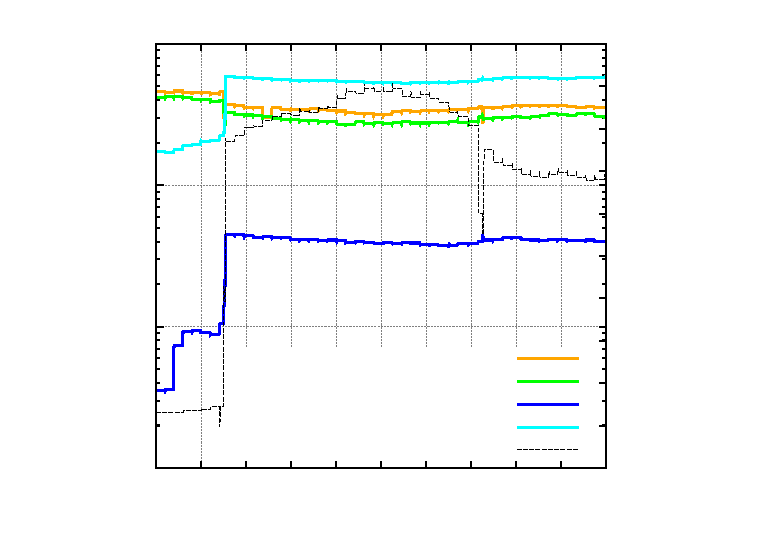
\includegraphics{eval_betweenness}}%
    \gplfronttext
  \end{picture}%
\endgroup

    \caption{Betweenness centrality of PolderCast and Scribe}
    \label{fig:eval_betweenness}
\end{figure}
